\section{Speed evaluation}
\label{sec:results:speed}

\subsection{Overall speed}

The full pipeline took 42s to process a video composed of 1000 frames, thus resulting in a speed of 38 FPS, higher than what was required.
To avoid waiting times due to the camera frame rate, these measurements were computed by using a video previously captured and saved as set of frames on the disk.

\subsection{Speed of the pipeline steps}

As visible in figure~\ref{fig:speed:all-pipeline}, the process is 2.3x as fast as the initial SMA-RTY implementation, which was already faster than the provided MATLAB script.
Naturally, the last step to complete is the last one of the pipeline, the \link*: however, as the next sections will show, the bottleneck is in the \locate* step.

\begin{figure}
	\centerline{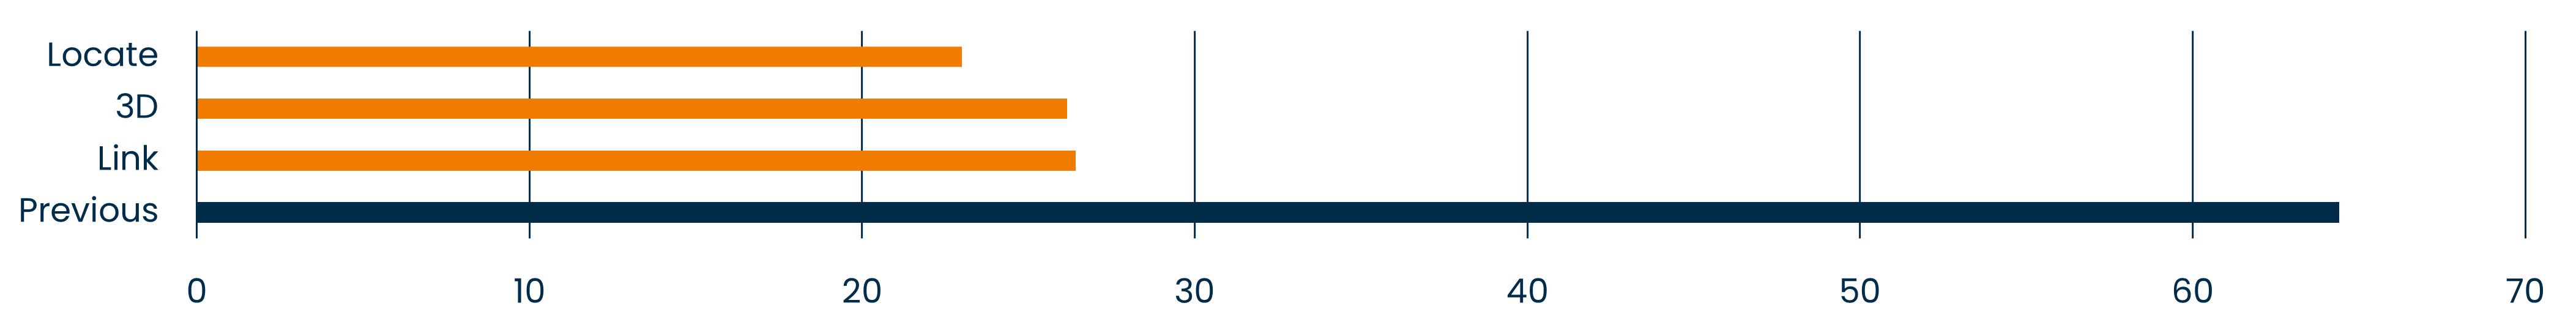
\includegraphics[width=\textwidth]{images/speed/overall-speed.png}}
	\caption{\centering The time required (in seconds) by the different pipeline steps to process a 1000-frames video}
	\label{fig:speed:all-pipeline}
\end{figure}

\subsubsection{\locate* step}

As shown in figure~\ref{fig:speed:locate}, the \locate* step was always fully operational, without ever having to wait for data.
This is obvious, since its input was already fully available at the start of the execution.
It must however be noted that, as visible in figure~\ref{fig:speed:all-pipeline}, the \locate* step did not finish much earlier than the others, indicating that it does not have a speed advantage over the other steps.

As visible in figure~\ref{fig:speed:locate}, the main bottleneck within this step is the time required for loading the images from the HDD to the RAM, to start processing them.

\begin{figure}
	\centerline{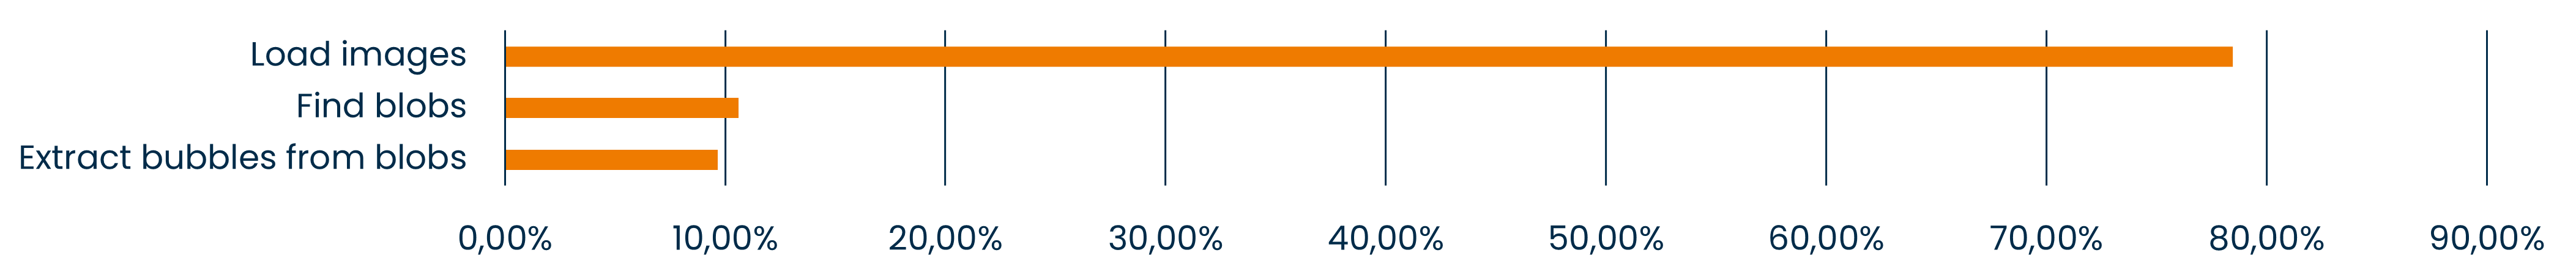
\includegraphics[width=\textwidth]{images/speed/locate.png}}
	\caption{\centering Distribution of how the \locate* step spent its execution time}
	\label{fig:speed:locate}
\end{figure}

\subsubsection{\match* step}

The \match* step, as visible in figure~\ref{fig:speed:match}, requires to spend a small amount of time waiting for the \locate* data.
This means that the \match* step is not the bottleneck.
The waiting time is however not extensive, indicating that even small slowdowns may make this step the bottleneck, affecting the whole pipeline performance.

\begin{figure}
	\centerline{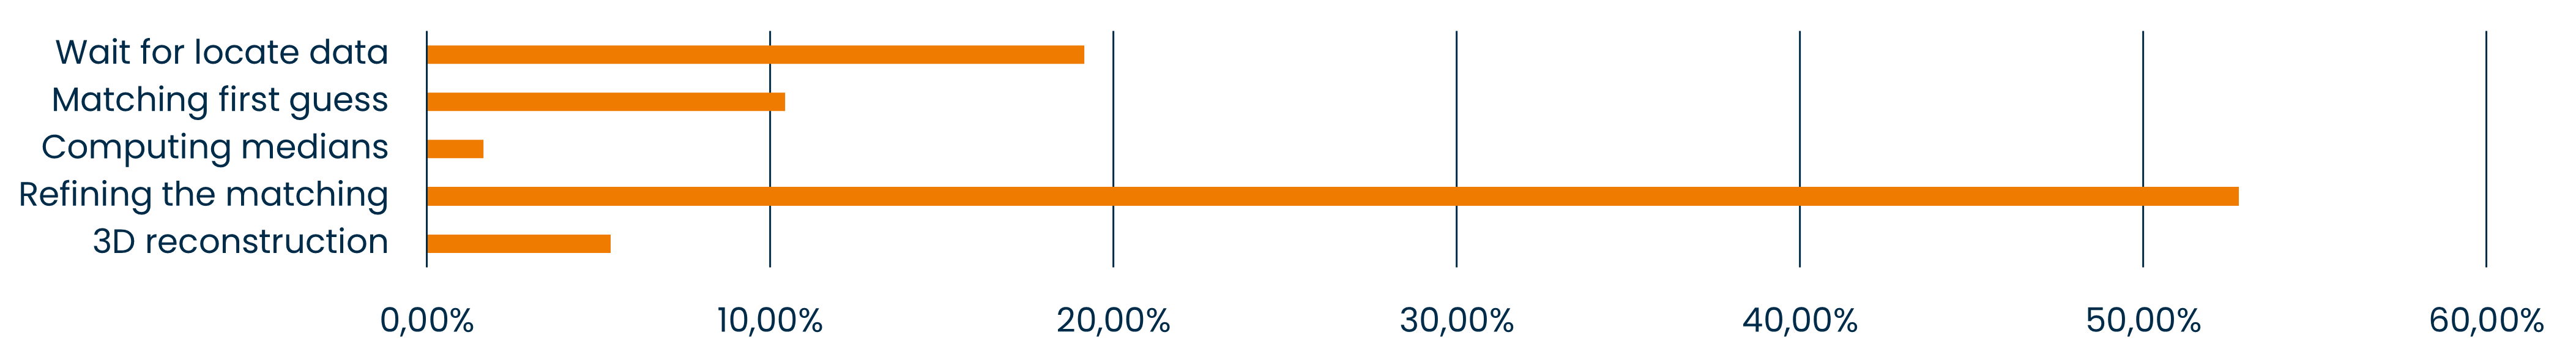
\includegraphics[width=\textwidth]{images/speed/matching.png}}
	\caption{\centering Distribution of how the \match* step spent its execution time}
	\label{fig:speed:match}
\end{figure}

\subsubsection{\link* step}

Figure~\ref{fig:speed:link} shows that most of the time the \link* step is idling, waiting for new inputs to be processed.
This indicates that it is far from being the bottleneck, and potentially more complex algorithm could be used instead, if they provided better results.

\begin{figure}[H]
	\centerline{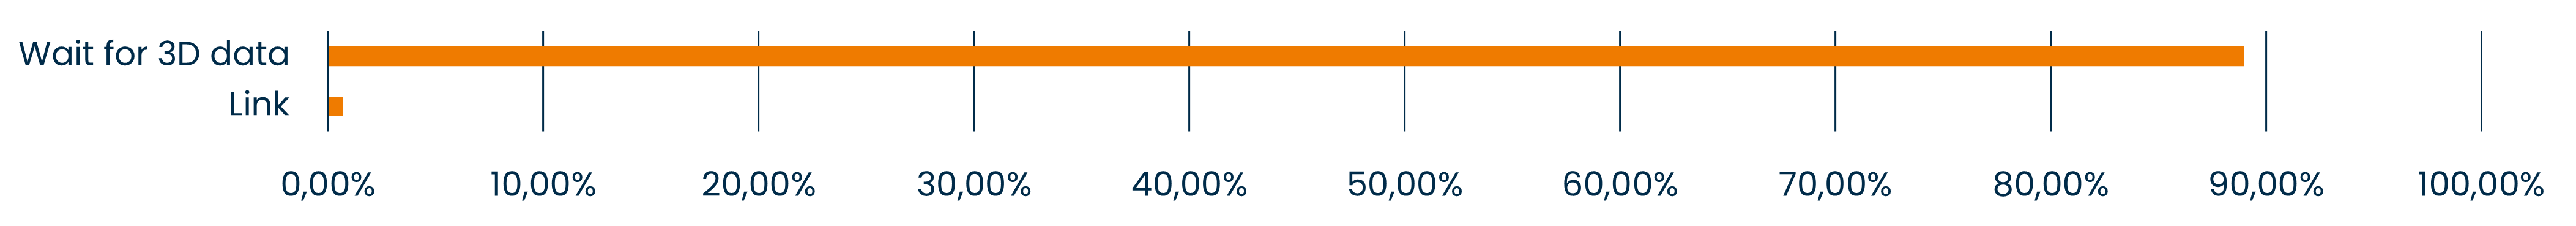
\includegraphics[width=\textwidth]{images/speed/link.png}}
	\caption{\centering Distribution of how the \link* step spent its execution time}
	\label{fig:speed:link}
\end{figure}

\subsection{Bottleneck evaluation}

As highlighted by the previous sections, the \locate* step is the current bottleneck of the system.
Figure~\ref{fig:pipeline-timing-schema} confirms this, by showing in a graphical way the timing of the different steps: the various \match* frames require to wait some time for the previous \locate* batches, and the \link* frames are constantly waiting for the \locate* output.

\begin{figure}[H]
	\centerline{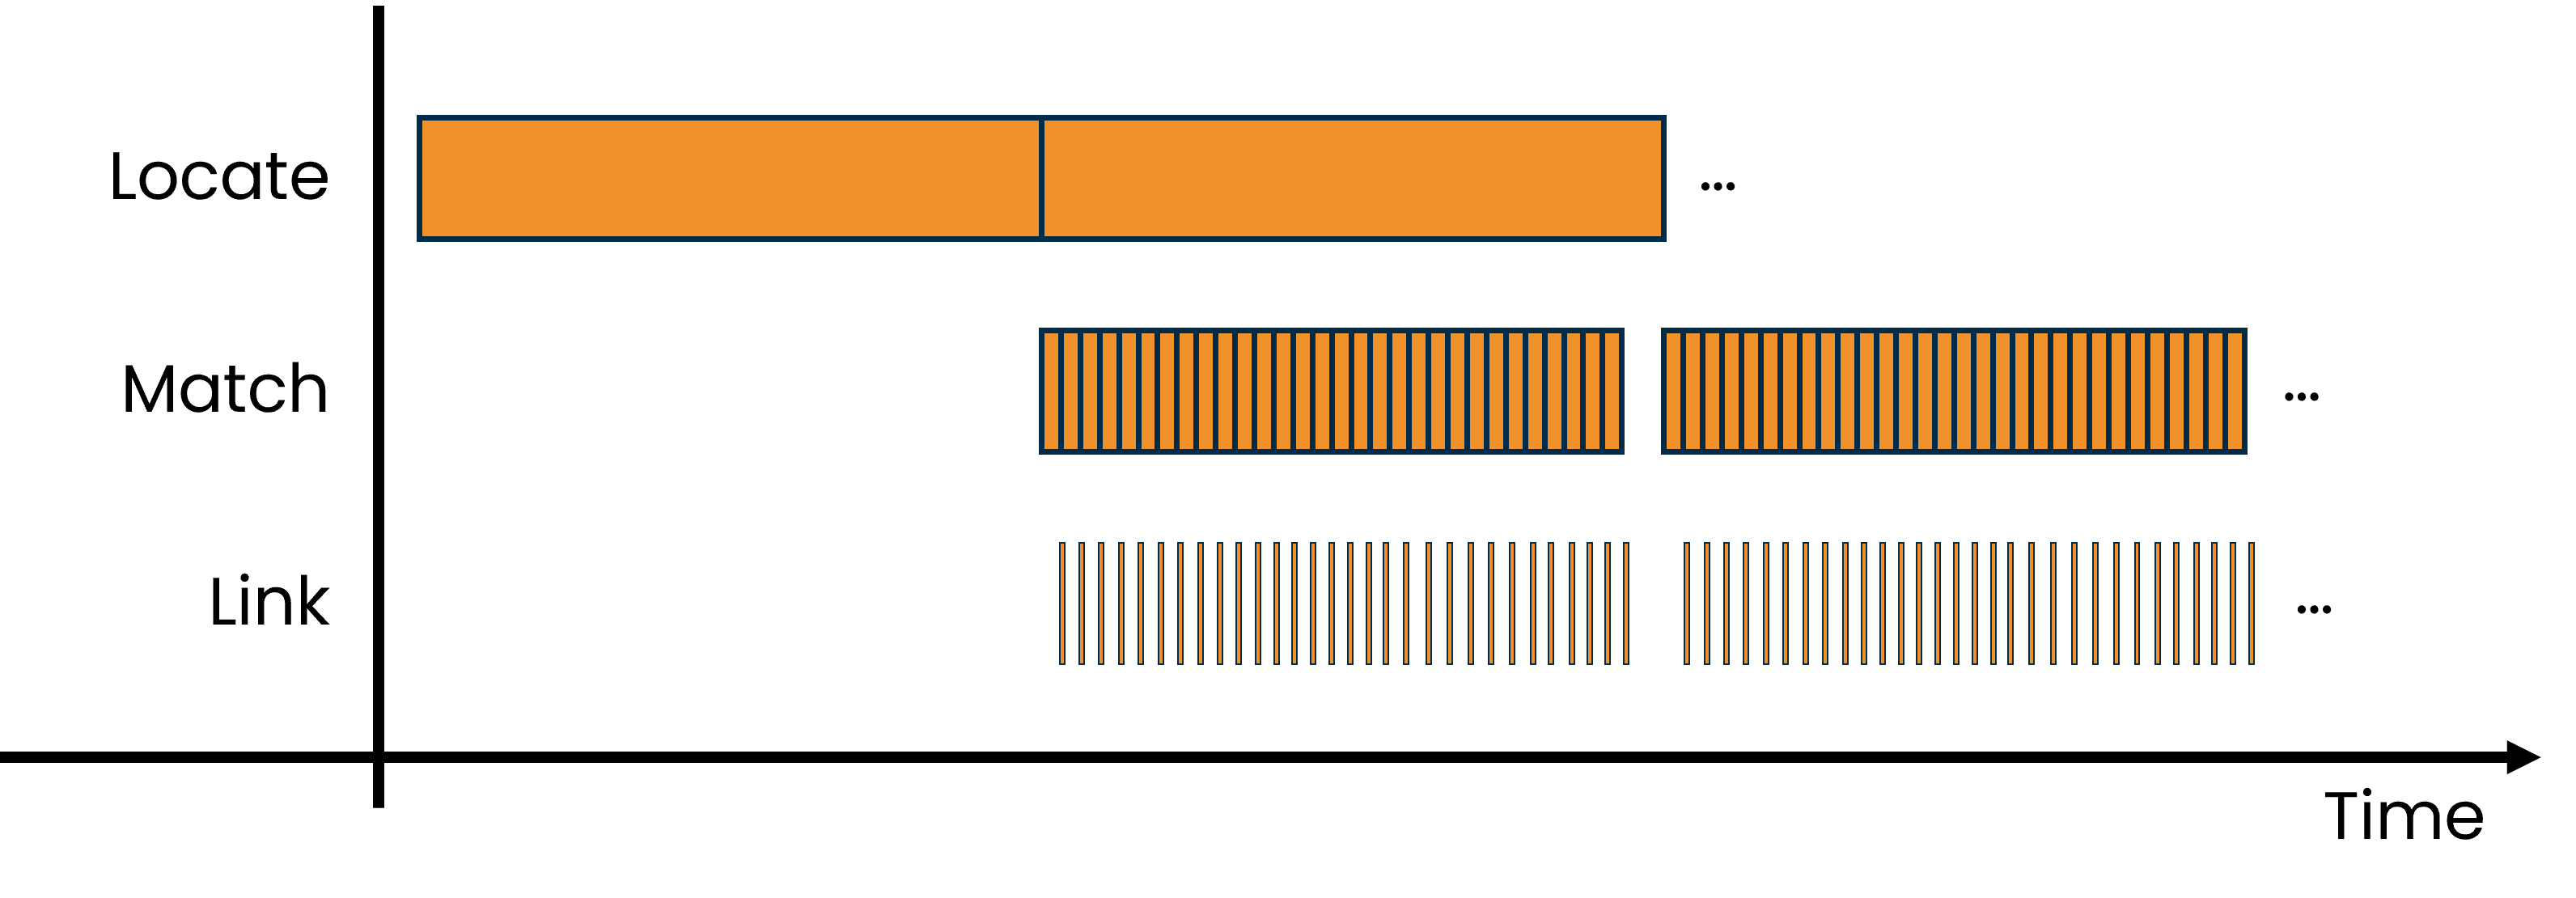
\includegraphics[width=.8\textwidth]{images/pipeline-timing.png}}
	\caption{\centering Schema (not to scale) of how the different pipeline stages are executed over time. The different rectangles indicate a batch of 20 frames per camera in the \locate*, and single frames in the other steps}
	\label{fig:pipeline-timing-schema}
\end{figure}
\newpage
